\documentclass[11pt]{standalone}
\usepackage{amssymb}
\usepackage{amsmath}
\usepackage[no-math]{fontspec}
\usepackage{unicode-math}
\usepackage{libertinus}
\usepackage{pgf,xcolor}
\usepackage{tikz}
\usetikzlibrary{arrows.meta, backgrounds, calc}
\usepackage{pgfplots}
\pgfplotsset{compat=newest}

\definecolor{my_darkgray}{HTML}{484949}
\definecolor{my_lightgray}{HTML}{F3F4F4}
\definecolor{my_darkblue}{HTML}{005A94}
\definecolor{my_lightblue}{HTML}{CCDEE9}
\definecolor{my_yellow}{HTML}{FFEC7F}
\definecolor{my_red}{HTML}{E60000}
\definecolor{my_orange}{HTML}{E87846}

\begin{document}
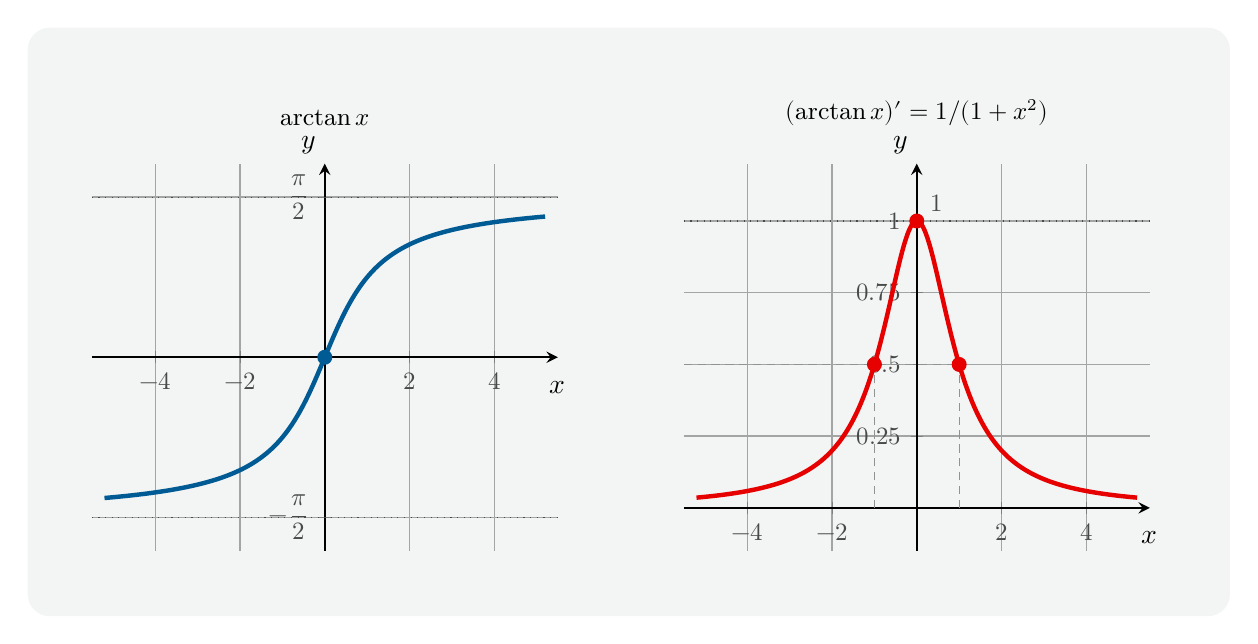
\begin{tikzpicture}[
    show background rectangle,
    background rectangle/.style={fill=my_lightgray, rounded corners=8pt},
    inner frame sep=0.8cm
]

% ── Left plot: arctan(x) ────────────────────────────────────────────────────
% Domain ℝ; range (-π/2, π/2) open – horizontal asymptotes at ±π/2.
% axis equal omitted: consistent with all other two-panel derivative figures.
\begin{axis}[
    name=left plot,
    axis lines = center,
    xlabel = {$x$},
    ylabel = {$y$},
    xlabel style = {at={(axis cs:5.5,0)}, anchor=north, yshift=-5pt},
    ylabel style = {anchor=south east},
    title = {$\arctan x$},
    title style = {font=\small, text=black, yshift=4pt},
    grid = both,
    grid style = {line width=0.3pt, draw=my_darkgray!30},
    major grid style = {line width=0.5pt, draw=my_darkgray!50},
    axis line style = {thick},
    xmin = -5.5, xmax = 5.5,
    ymin = -1.9, ymax = 1.9,
    xtick = {-4,-2,0,2,4},
    ytick = {-1.5708, 0, 1.5708},
    yticklabels = {$-\dfrac{\pi}{2}$, $0$, $\dfrac{\pi}{2}$},
    yticklabel style = {font=\small, text=my_darkgray},
    xticklabel style = {font=\small, text=my_darkgray},
    width=7.5cm, height=6.5cm,
    clip=true,
]

% Horizontal asymptotes at y = ±π/2: range is open interval
\foreach \ya in {-1.5708, 1.5708}{
    \addplot[draw=my_darkgray, dotted, thin, domain=-5.5:5.5]{ \ya };
}

% arctan(x) on all of ℝ
\addplot[
    draw=my_darkblue,
    samples=500,
    ultra thick,
    domain=-5.2:5.2
]{ atan(x) * pi / 180 };

% Mark the inflection point (0, 0) where the maximum slope occurs
\addplot[
    mark=*,
    mark size=2.5pt,
    only marks,
    draw=my_darkblue,
    fill=my_darkblue
] coordinates {(0, 0)};

\end{axis}

% ── Right plot: (arctan x)' = 1/(1 + x²) ───────────────────────────────────
% Domain ℝ; no singularities. Range (0, 1]: maximum 1 at x = 0,
% decaying to 0 as |x| → ∞.
\begin{axis}[
    name=right plot,
    at={($(left plot.east)+(1.6cm,0)$)},
    anchor=west,
    axis lines = center,
    xlabel = {$x$},
    ylabel = {$y$},
    xlabel style = {at={(axis cs:5.5,0)}, anchor=north, yshift=-5pt},
    ylabel style = {anchor=south east},
    title = {$(\arctan x)' = 1/(1+x^2)$},
    title style = {font=\small, text=black, yshift=4pt},
    grid = both,
    grid style = {line width=0.3pt, draw=my_darkgray!30},
    major grid style = {line width=0.5pt, draw=my_darkgray!50},
    % axis equal omitted: y range 0..1 vs x range ±5 – very different scales
    axis line style = {thick},
    xmin = -5.5, xmax = 5.5,
    ymin = -0.15, ymax = 1.2,
    xtick = {-4,-2,0,2,4},
    ytick = {0, 0.25, 0.5, 0.75, 1.0},
    yticklabel style = {
        /pgf/number format/fixed,
        /pgf/number format/precision=2,
        font=\small,
        text=my_darkgray
    },
    xticklabel style = {font=\small, text=my_darkgray},
    width=7.5cm, height=6.5cm,
    clip=true,
]

% Dotted horizontal line at y = 1: maximum value at x = 0
\addplot[draw=my_darkgray, dotted, thin, domain=-5.5:5.5]{ 1 };
\node[anchor=south west, font=\small, text=my_darkgray]
    at (axis cs:0.1, 1) {$1$};

% 1/(1 + x²): smooth on all of ℝ, no singularities
\addplot[
    draw=my_red,
    samples=500,
    ultra thick,
    domain=-5.2:5.2
]{ 1 / (1 + x^2) };

% Mark the maximum (0, 1)
\addplot[
    mark=*,
    mark size=2.5pt,
    only marks,
    draw=my_red,
    fill=my_red
] coordinates {(0, 1)};

% Mark (1, 0.5) and (-1, 0.5): 1/(1+1) = 0.5, showing the decay rate
\addplot[
    mark=*,
    mark size=2.5pt,
    only marks,
    draw=my_red,
    fill=my_red
] coordinates {(-1, 0.5) (1, 0.5)};

% Drop lines from (±1, 0.5) to both axes
\foreach \xa in {-1, 1}{
    \addplot[draw=my_darkgray!60, densely dashed, thin]
        coordinates {(\xa, 0) (\xa, 0.5)};
}
\addplot[draw=my_darkgray!60, densely dashed, thin]
    coordinates {(-5.5, 0.5) (1, 0.5)};

\end{axis}

\end{tikzpicture}
\end{document}
